%------------------------------------------------------------------------------
\ifpdf
\graphicspath{{bild/}}
%{80_Bilder/PDF/}
%{80_Bilder/}}
\else
\graphicspath{%{80_Bilder/EPS/}
	%{80_Bilder/}
	{bild/}}
\fi
%%%%%%%%%%%%%%%%%%%%%%%%%%%%%%%%%%%%%%%%%%%%%%%%%%%%%%%%%%%%%%%%%%%%%%
%%%%%%%%%%%%%%%%%%%%%%%%%%%%%%%%%%%%%%%%%%%%%%%%%%%%%%%%%%%%%%%%%%%%%%
\chapter{Reglerentwurf durch Trajektorieplanung}
\label{ch:Reglerentwurf-durch-Trajektorieplanung}
In diesem Kapitel werden einige Regler für die sogenannten unteraktuierten Systeme entworfen, welchedie Brockett-Bedingung nicht erfüllen. Im Abschnitt \ref{sec:Unteraktuiertes_mechanisches_System} werden die Definition und der Charakter vom Unteraktuierten mechanischen System ausgegeben. Der Entwurf von Steuergesetze mit und ohne die Trajektorieplanung aus \emph{PyTrajectory} werden separat in Abschnitt \ref{sec:Reglerentwurf_mittels_PyTrajectory} vorgestellt.

\section{Unteraktuierte mechanische Systeme}
\label{sec:Unteraktuiertes_mechanisches_System}
Unter einem unteraktuierten mechanischen System (UMS) versteht man ein spezielles System mit weniger unabhängigen Aktuatoren als der Anzahl von Freiheitsgrade. Im Vergleich mit einem vollständig aktuierten System kann ein UMS mittels weniger Eingängen ggf. gleiche Aufgabe lösen. Aufgrund der Dynamik des Systems oder zur Reduzierung der Kosten sind UMS in vielen Bereichen verbreitet.

Für die Bestimmung von Bewegungsabläufen eines Körpers relativ zu einem Inertialsystem nennt man die konstruktiv geometrischen oder mechanischen Einschränkungen der Pose oder Geschwindigkeit an den Körper \emph{Zwangsbedingungen}.

Eine holonome Zwangsbedingung beschränkt die Position oder Geschwindigkeit des Körpers, die durch algebraische Gleichungen oder \emph{integrierbare} Differenzialgleichungen dargestellt wird. Im Gegenteil dazu enthält eine nichtholonome Zwangsbedingung nicht integrierbare Differenzialgleichungen. Mit anderen Worten verfügt eine holonome Zwangsbedingung über die Form wie: $f(x,y,z,t)=0$ und eine nichtholonome über die Form wie: $g(x,y,z,\dot{x},\dot{y},\dot{z},t)=0$ (die Ableitung kann nicht in der Form von $f$ integriert werden).

Wenn die Systemgleichungen die Form $h(x,y,z,\dot{x},\dot{y},\dot{z},\ddot{x}, \ddot{y}, \ddot{z}, t) = 0$ besitzen, werden sie je nach Integrierbarkeit als \emph{holonome} oder \emph{nichtholonome Zwangsbedingung zweiter Ordnung} \cite{oriolo1991control} bezeichnet. Wenn $h$ in die Form $g(x,y,z,\dot{x},\dot{y},\dot{z},t)=0$ integriert werden kann, heißt $h$ eine \emph{partiell integrierbare} Zwangsbedingung. Wenn $h$ zwei mal mit der Schlussform $f(x,y,z,t)=0$ integriert werden kann, heißt das \emph{vollständig integrierbare} System holonomes System.

Der Freiheitsgrad eines Systems mit $n_{r}$ redundanten Koordinaten und $n_{ZB}$ holonomen Zwangsbedingungen ist $n=n_{r}-n_{ZB}$. Die Minimalkoordinate $\vect{q}=(q_{1},q_{2},...,q_{n})^{T}$ beschreibt dann die Konfiguration des Systems.

Zur Beschreibung der kinetischen Charakteristik nimmt man mit der EULER-LAGRANGE-Gleichungen nach \cite{janschek2009systementwurf}: 
\begin{eqnarray}
&~&L(\vect{q},\dot{\vect{q}}) = T^{\ast}(\vect{q},\dot{\vect{q}})-V(\vect{q}) = \frac{1}{2}\dot{\vect{q}}^{T}\matr{M}(\vect{q})\dot{\vect{q}}-V(\vect{q})\text{~~~~~~~~~(LAGRANGE-Funktion)}\notag\label{eq:LAGRANGE-Funktion}\\
\\
&~&\frac{\mathrm{d} }{\mathrm{d} t}\frac{\partial L(\vect{q},\dot{\vect{q}})}{\partial \dot{q}_{i}}- \frac{\partial L(\vect{q},\dot{\vect{q}})}{\partial q_{i}} = f_{i}, ~~~~~~i = 1,\ldots, N.~~~~~~~~~~~\text{(EULER-LAGRANGE-Gln.)}\notag\label{eq:EULER-LAGRANGE-Gln.}\\
\end{eqnarray}
an. Gl. \eqref{eq:LAGRANGE-Funktion} gibt die Darstellung von der kinetischen Koenergie $T^{\ast}$ und der potenziellen Energie $V$. In Gl. \eqref{eq:EULER-LAGRANGE-Gln.} steht $f_{i}$ für die bezüglich der Koordinate $q_{i}$ eingeprägten und externen Kräften. Die Massen-/Trägheitsmatrix $\matr{M}$ ist symmetrisch und positiv definit.

Durch die Umformung von Gl. \eqref{eq:EULER-LAGRANGE-Gln.} in Vektorform erhält man \cite{olfati2001nonlinear}:
\begin{eqnarray}
\matr{M}(\vect{q})\ddot{\vect{q}} + \matr{C}(\vect{q},\dot{\vect{q}})\dot{\vect{q}} + \matr{G}(\vect{q}) = \vect{F}(\vect{q})\label{eq:Vectorform_EULER-LAGRANGE-Gln.}
\end{eqnarray}
wobei Matrix $\matr{C}$ die Wirkung von Zentrifugal- bzw. Corioliskraft und Matrix $\matr{G}$ konservative Kraft wie Gravitation darstellt.

Falls $rank(\vect{F}) = m \stackrel{!}{=} n$ heißt das System \emph{vollständig aktuiertes} System. Wenn $m < n$ wird das System unter \emph{unteraktuiertes} System genannt. Die Koordinaten $\vect{q}$ in einem UMS können in die vom Eingang $\vect{F}$ beeinflussten $\vect{q_{a}}$ und nicht beeinflussten $\vect{q_{u}}$ Koordinaten aufgeteilt werden: $\vect{q} =  [\vect{q_{a}},\vect{q_{u}}]^T$ mit $\vect{q_{a}}=(q_{1},\cdots,q_{m})^{T}$ und $\vect{q_{u}} = (q_{m+1},\cdots,q_{n})^{T}$. Ausgehend davon kann Gl. \eqref{eq:Vectorform_EULER-LAGRANGE-Gln.} in die folgende Form aufteilen:
\begin{eqnarray}
\begin{bmatrix}
\matr{M}_{a}\\ \matr{M}_{u}
\end{bmatrix}\begin{bmatrix}
\ddot{\vect{q}}_{a}\\\ddot{\vect{q}}_{u} 
\end{bmatrix} + \begin{bmatrix}
\matr{C}_{a}\\\matr{C}_{u} 
\end{bmatrix}\begin{bmatrix}
\dot{\vect{q}}_{a}\\\dot{\vect{q}}_{u}
\end{bmatrix} + \begin{bmatrix}
\matr{G}_{a}\\\matr{G}_{u}
\end{bmatrix} = \begin{bmatrix}
\vect{u}_{a}\\ \vect{0} 
\end{bmatrix}.\label{eq:aufgeteilt_EULER-LAGRANGE-Gln.}
\end{eqnarray}
Die erste Zeile in Gl. \eqref{eq:Vectorform_EULER-LAGRANGE-Gln.} bezeichnet man als aktuiertes Subsystem und die zweite Zeile unaktuiertes Subsystem, die auch als eine Zwangsbedingung zweiter Ordnung betrachtet werden kann. Gemäß \cite{oriolo1991control} gehört die zweite Zeile zur nichtholonomen Zwangsbedingungen zweiter Ordnung. Nach \cite{spong1995swing} kann man bei der Linearisierung von System mit Systemfunktionen wie Gl. \eqref{eq:aufgeteilt_EULER-LAGRANGE-Gln.} $\ddot{\vect{q}_{a}}$ als den Eingangsvektor $\vect{v}$ wählen, damit sich der originale Systemeingang $\vect{u}$ als die Form von Systemzustandsvektor und $\vect{v}$ darstellen lässt. Aus diesem Grund wird die Wagenverschiebung $x_{1}$ in Beispiel \ref{bp:Inverses_Pendel_System} als der virtuelle Systemausgang ausgewählt.

\section{Reglerentwurf mittels \emph{PyTrajectory}}
\label{sec:Reglerentwurf_mittels_PyTrajectory}
Mit dem Paket \emph{PyTrajectory} kann eine Trajektorie durch Lösung einer Randwertaufgabe geplant werden. Die Idee ist es, durch die Analyse der entworfenen Trajektorien für $\vect{u}_{t}$ in der Umgebung einer Ruhelage ein Steuergesetz zu konstruieren und zwar für Systeme, die die Brockett-Bedingung nicht erfüllen.

Man kann die Umgebung $M$ als eine Scheibe/ein Quadrat oder eine Kugel/einen Würfel betrachten, wenn die Anzahl der Systemzustände $2$ oder $3$ ist. Einige typischen Punkte werden daraus als die Anfangspunkte der Trajektorien ausgewählt. Die Trajektorieplanung wird durch \emph{PyTrajectory} durchgeführt. Aus der Regelmäßigkeit der Trajektorien kann man dann versuchen, ein Steuergesetz zu finden.   

Das erste Modell ist der nicht-holonome Doppelintegrator von Brockett. 

\subsection{Ausgang: Brocketts nicht holonomen Doppelintegrator}
\label{subs:Ausgang_Brocketts_nicht_holonimischer_Doppelintegrator}
Das berühmte unteraktuierte Beispiel von Brockett wurde schon im Abschnitt \ref{Erläuterung_zur_Brockett-Bedingung}, Beispiel \ref{bp:Brocketts_Doppelintegrator} vorgestellt:
\begin{eqnarray}
\dot{x}_{1} &=& u_{1}\notag\\
\dot{x}_{2} &=& u_{2}\notag\\
\dot{x}_{3} &=& x_{2}u_{1}-x_{1}u_{2}.
\label{eq:Brockett_Doppelintegrator_ch4}
\end{eqnarray}
Der Freiheitsgrad dieses Systems ist $n=3$ während es nur $m=2$ Eingänge gibt. Damit ist es ein unteraktuiertes System. Wegen $\mathrm{rang{(\vect{x})}=3}$ wählt man einen Würfel mit der Länge der Seite $0.2$ als die Umgebung von $\vect{0}$ (siehe Abb. \ref{fig:Asy_plot}). Die Ruhelage liegt gerade um den Mittelpunkt und die typischen Anfangspunkte (oder als \emph{Testpunkte} genannt) bestehen aus den acht Ecken, zwölf Mittelpunkten der Kanten, sechs Mittelpunkten der Begrenzungsflächen. 

\begin{figure}
	\centering
	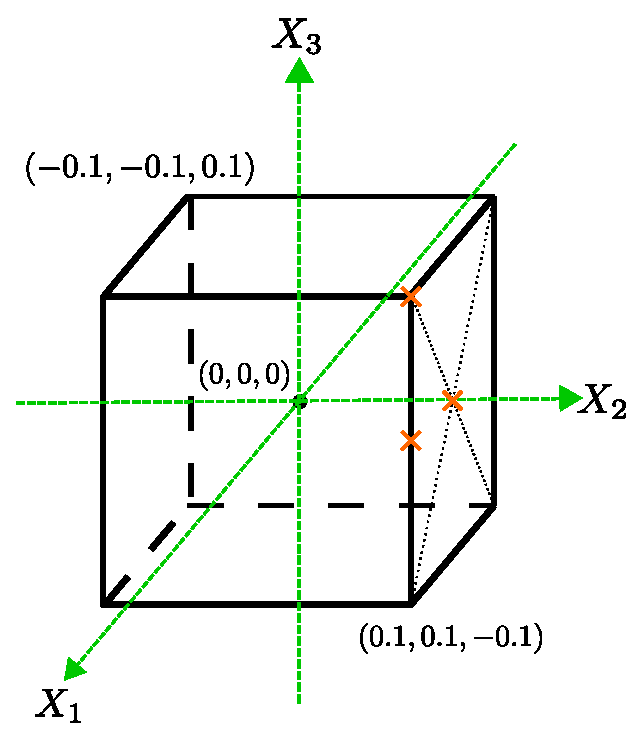
\includegraphics[width=0.35\linewidth]{bild/modul/Asy_plot.eps}%6cm
	\caption{Skizze des Würfels als die Umgebung von der Ruhelage. Die orange Kreuze sind die ausgewählten Anfangspunkte in einer Quadrate.}
	\label{fig:Asy_plot}
\end{figure}

Für dieses Beispiel werden einige Methoden zum Entwurf der Trajektorien von $\vect{u}$ und dann $\vect{x}$ angewendet. Die erste Methode ist noch der Kollokationsverfahren mittels \emph{PyTrajectory}. 

\subsubsection{Trajektorienplanung mit \emph{PyTrajectory}}
Die Einstellung von \emph{PyTrajectory} ist wie folgt: Anfangswerte von freien Parameter $\vect{c}_{f}$ für Spline-Abschnitte sind $0.1$, der Anfangsschätzwert von $k$ ist $1.0$, der Anfangszahl und das Vielfache für den Spline-Abschnitt in der nächsten Iteration ist jeweils $2$.


Mit \emph{PyTrajectory} wird eine Trajektorie von $\vect{u(t)}$ für jeden Ausgangspunkt geplant. Verschiedene Testpunkte benötigen verschiedene Iteration-Mal zwischen $1$ und $3$. Da die Randwerte der Straffunktion sind $k_{min}=0.1$ und $k_{max}=5.0$ gewählt, schwingt der Wert von $k_{end}$ bei unterschiedliche Testpunkte um $2.5$. Abb. \ref{fig:Trajektorien_von_u_1_aus_PyTrajectory} und \ref{fig:Trajektorien_von_u_2_aus_PyTrajectory} zeigen die Simulationskurven der Eingangstrajektorien, die aber keine deutliche Regelmäßigkeit besitzen\footnote{Regelmäßigkeit hier bedeutet, dass die Kurven ca. die gleiche Form besitzen.}\footnote{Zum besser Lesen werden nur fünf Kurven angezeigt. Die gesamten Kurven sind in Abb. \ref{fig:Eingangsverlauf_u1} und \ref{fig:Eingangsverlauf_u2} dargestellt.}. Die Tabelle in dem Anhang \ref{tab:Pytra_Asy_Brockett_Doppelintegrator} beschreibt die Details der Trajektorienkurven. Die Form der Kurven hängt nicht direkt von den Ausgangspunkten ab. In diesem Beispiel werden die Startwerte der Systemzustände gleichzeitig verändert, was die Findung einer Regelmäßigkeit erschwert. Deshalb wird als nächster Schritt die Regelmäßigkeit der Kurven bei der Veränderung nur eines Zustands untersucht.

\begin{figure}[!h]
	\centering
		\includegraphics[width=0.8\linewidth]{bild/30_32/Brockett_e2_Asy_PyTrajectory_d_01_u1.pdf}%12cm
	\caption{Eingangsverläufe $u_{1}$ mit verschiedenen $\vect{x}_{0}$ für Brocketts nicht-holonomen Doppelintegrator mittels \emph{PyTrajectory}.}
	\label{fig:Trajektorien_von_u_1_aus_PyTrajectory}
\end{figure}

\begin{figure}[!h]
	\centering
	\includegraphics[width=0.8\linewidth]{bild/30_32/Brockett_e2_Asy_PyTrajectory_d_01_u2.pdf}%12cm
	\caption{Eingangsverläufe $u_{2}$ mit verschiedenen $\vect{x}_{0}$ für den Brocketts nicht-holonomen Doppelintegrator mittels \emph{PyTrajectory}.}
	\label{fig:Trajektorien_von_u_2_aus_PyTrajectory}
\end{figure}

\textbf{Testpunkte von $x_{1}$ verändert von $-0.1$  bis zu $-0.01$}~~Zuerst wählt man, die Anfangspunkte von $x_{1}$ von $-0.1$ bis zu $-0.01$, mit der Schrittweite $\Delta x_{1} = 0.01$. Die Anfangswerte von $x_{2}$ und $x_{3}$ bleiben in den $10$ Situationen immer $0.1$. 

\begin{figure}[!h]
	\centering
	\begin{subfigure}[c]{\textwidth}
		\centering
		\label{fig:Pytra_x1_-0.09_0.0_deltax=0.01_x_1}
		\includegraphics[width=0.9\linewidth]{bild/30_32/Brockett_e2_local/Pytra_x1_-009_00_deltax=001_x.pdf}
		%\subcaption{Die berechnete Ergebnisse von $\vect{x}$.}	
	\end{subfigure}\\
	%\hspace{-1in} %0.5\textwidth
	\begin{subfigure}[c]{\textwidth}
		\centering
		\label{fig:Pytra_x1_-0.09_0.0_deltax=0.01_x_3}
		\hspace*{-1.7cm}
		\includegraphics[width=0.85\linewidth]{bild/30_32/Brockett_e2_local/Pytra_x1_-009_00_deltax=001_x_3.pdf}
		%\subcaption{Die berechnete Ergebnisse von $u$ und $k$.}
	\end{subfigure}
	\caption{Zustands- und Eingangsverläufe des Doppelintegrator-Systems.}
	\label{fig:Pytra_x1_-0.09_0.0_deltax=0.01_x}
\end{figure}

\begin{figure}[!h]
	\centering
	\includegraphics[width=0.9\linewidth]{bild/30_32/Brockett_e2_local/Pytra_x1_-009_00_deltax=001_u.pdf}%15.5cm
	\caption{Eingangsverläufe mit den Anfangswerten von $x_{1}$ zwischen $-0.10$ und $-0.01$.}
	\label{fig:Pytra_x1_-0.09_0.0_deltax=0.01_u}
\end{figure}

Jeder Fall braucht $2$ oder $3$ Iterationen mit $k_{end}$ zwischen $2.0-2.7$. Wie Abb. \ref{fig:Pytra_x1_-0.09_0.0_deltax=0.01_u} darstellt, geht die Amplitude der ``minus Sinuskurven'' von $u_{1}$ mit der Steigerung von $x_{1,0}$ im Bereich von $(-0.1, -0.03)$ (außer des Falls bei $x_{1,0}=-0.08$) immer herunter, während sich die Amplitude der sinusförmigen Kurve von $u_{2}$ immer vergrößert. Das heißt, in diesem Bereich ergeben sich beide Systemeingänge eine ähnliche Trajektorienform. Über $-0.02$ verkleinert die Amplitude der Kurven sehr schnell zu ungefähr $-1$. (Die Kurven von $-0.02$ und $-0.01$ liegen so nahe, dass nur eine Linie im Bild zu sehen ist. Dieser Effekt tritt z.B. auch bei $x_{3}$ in Abb. \ref{fig:Pytra_x1_-0.09_0.0_deltax=0.01_x} in den Situationen $(-0.08, -0.02,-0.01)$.

Die Zustandverläufe verfügen bei der separaten Veränderung von $x_{2,0}$ und $x_{3,0}$ jeweils in einem kleinen Bereich über auch eine Regelmäßigkeit. Aber wenn die Anfangswerte zwei der drei Systemzustandsvariable gleichzeitig verändert werden, ergeben die Trajektorien keine bestimmte Änderungsregelmäßigkeit. 

Die Trajektorien zeigen eine Regelmäßigkeit in einem kleinen Bereich in dem Brocketts nicht-holonomen System, das die Brockett $2.$ Bedingung nicht erfüllt. Ob diese Regelmäßigkeit auch für das inversen-Pendel-System geeignet ist, lässt sich im nächsten Abschnitt untersuchen. 

\subsection{Eingangsverlauf des inverse-Pendel-Systems}
\label{Ausgang_Das_inverse_Pendel_System}
Die Zustandsfunktion des Benchmark-Systems erfüllt wegen des surjektiven Bildwerts die Brockett $2.$Bedingung. Erinnert man die Gl. \eqref{eq:DLG_Inverses_Pendel_partiell_lin} und lässt sich der Wert von $x_{1}$ von $-1.0$ mit der Schrittweite $h=0.1$ bei jedem Fall zu $-0.4$ vergrößern.

Mit dem Ergebnis in Abb. \ref{fig:Inverses_Pendel_Asy_x1_-10_-04_u} zeigt die Kurven eine ähnliche Regelmäßigkeit wie zuvor: mit Anfangswerte von $x_{1}$ in einem begrenzten Raum ($-1.0,-0.5$) kann man den Linientrend schätzen, außerhalb davon verändert die Kurve mit eine ganz verschiedene Form plötzlich. 
\begin{figure}[!h]
	\centering
	\includegraphics[width=0.95\linewidth]{bild/30_32/Inverses_Pendel_Asy_x1_-10_-04_u.pdf}%15.5cm
	\caption{Eingangsverläufe mit den Anfangswerten von $x_{1}$ zwischen $-1.0$ und $-0.4$.}
	\label{fig:Inverses_Pendel_Asy_x1_-10_-04_u}
\end{figure} 

 In anderen Simulationen, wo $x_{2,0}$ zwischen $(0.2,2.9)$ verändert und $x_{1,0}=x_{4,0}=0, x_{3,0}=\pi$ ist, besitzen alle Trajektorien auch ähnliche Form. Aber die Kombination der obere Untersuchungen, nämlich lässt $x_{1,0}$ und $x_{2,0}$ jeweils in dem Bereich $(-1.0,-0.5)$ und $(0.2,2.9)$ gleichzeitig annehmen, bleiben die Trends alle Kurven nicht identisch (wie Abb. \ref{fig:Inverses_Pendel_Asy_x1_-1_-05_x2-02_30_u}).
\begin{figure}[!h]
	\centering
	\includegraphics[width=0.95\linewidth]{bild/30_32/Inverses_Pendel_Asy_x1_-1_-05_x2-02_30_u.pdf}%15.5cm
	\caption{Eingangsverläufe mit den Anfangswerten von $x_{1}$ zwischen $-1.0$ und $-0.5$ und $x_{2}$ zwischen $0.2$ und $2.9$.}
	\label{fig:Inverses_Pendel_Asy_x1_-1_-05_x2-02_30_u}
\end{figure} 

Daraus ergibt sich die Konsequenz\footnote{Das System des zwei-Gelenken-Manipulators wird auch untersucht, dessen Ergebnis im Anhang \ref{Ausgang_Zwei_Gelenke_Manipulator} gezeigt ist.}: wenn die Anfangswerte von \textbf{nur einem Systemzustandskomponente} in einem \textbf{abgrenzten} Bereich abwandeln, besitzt die Amplitude und die Form der Trajektorienkurven mittels des Python-Pakets \emph{PyTrajectory} eine Regelmäßigkeit. Das gilt in dem System, egal es die Brockett $2.$ Bedingung erfüllt oder nicht. Unter dieser Voraussetzung kann man dann die Möglichkeit eines Steuergesetz $\vect{u(t)}$ überlegen.

\subsection{Entwurf des Steuergesetz mittels Trajektorien aus \emph{PyTrajectory}}
\label{Entwurf_des_Steuergesetz_mittels_Trajektorien_aus_PyTrajectory}
Da die Ueberfuehrungstrajektorien einen allmählich änderte Form in einem Bereich besitzen, ist es möglich, einen Steuergesetz für den gesamten Bereich zu konstruieren. Mit \emph{PyTrajectory} kann im ersten Schritt jeweils eine Trajektorie für die Systemzustandsveränderung aus einigen Startposition in der Umgebung einer Ruhelage in die wie im letzten Abschnitt entworfen werden, dann werden die Trajektorien $\vect{u}_{t}$ mit Interpolation dieser bekannten Trajektorien erstellt.  

Aus Zeitgründen wird in der Arbeit nur ein sehr einfacher Fall vorgestellt: Entwurf des Steuergesetz mit unterschiedlichen $x_{1,0}$.

Wie in dem letzten Abschnitt gezeigt wird, wählt man den Veränderungsbereich von $x_{1,0}$ zwischen $(-0.07,-0.03)$ mit der Schrittweite $0.01$. Die bekannte $\vect{u}(t)$ von \emph{PyTrajectory} mit beispielsweise $p$ Zeitpunkten sind in einer List gespeichert. Die ausgesuchten Eingangstrajektorien mit z.B. $x_{1,0}=-0.043$ braucht zuerst die gehörenden Strecke nämlich einen Bereich zwischen $(-0.05,-0.04)$ zu finden. Damit die Größe der Trajektorie zu jedem Zeitpunkt $p_{i}$ kann mittels der Punkte in der Kurven mit $x_{1,0}=-0.05$ und $-0.04$ linear interpoliert.

Die Interpolationsergebnisse sind in Abb. \ref{fig:Brockett_e2_interpolation_u} und \ref{fig:Brockett_e2_interpolation_x} gezeigt. Nur drei der Trajektorien wurden aus \emph{PyTrajectory} vorgegeben, die anderen sieben sind dadurch interpoliert. In allen Fällen laufen Systemzustandsvariablen schließlich zu der Ruhelage. 
\begin{figure}[!h]
	\centering
	\includegraphics[width=0.8\linewidth]{bild/30_32/Brockett_e2_interpolation_u.pdf}%15.5cm
	\caption{Eingangsverlauf mit dem Anfangszustand von $x_{1}$ in $(-0.05,-0.04)$ mit Interpolation.}
	\label{fig:Brockett_e2_interpolation_u}
\end{figure} 

\begin{figure}[!h]
	\centering
	\includegraphics[width=\linewidth]{bild/30_32/Brockett_e2_interpolation_x.pdf}%15.5cm
	\caption{Zustandsverlauf mit dem Anfangszustand von $x_{1}$ in $(-0.05,-0.04)$ mit Interpolation.}
	\label{fig:Brockett_e2_interpolation_x}
\end{figure} 
 
\section{Trajektorienplanung mit Polynomform von $\vect{u}(t)$}
In diesem Abschnitt wird ein Steuergesetz für das Brockett Beispiel ohne Berücksichtigung der geplannten Trajketorien aus \emph{Pytrajectory} diskutiert. Zuerst wird eine Polynomform für die Systemeingänge aufgestellt, die die $2$. Bedingung von Brockett erfüllt.

Es wird angenommen, dass $u_{1}$ und $u_{2}$ jeweils ein Polynom der Zeit $t$ ist:
\begin{eqnarray}
u_{1} &=& a_{0}+a_{1}t+a_{2}t^{2}\notag\\
u_{2} &=& b_{0}+b_{1}t+b_{2}t^{2}.
\label{eq:Brocketts_Beispiel_u}
\end{eqnarray}
Integriert man die ersten zwei Gleichungen in Gl. \eqref{eq:Brocketts_Beispiel_u}, erhält man:
\begin{eqnarray}
x_{1} &=& a_{0}t +\frac{1}{2}a_{1}t^{2}+\frac{1}{3}a_{2}t^{3}+\alpha \notag\\
x_{2} &=& b_{0}t +\frac{1}{2}b_{1}t^{2}+\frac{1}{3}b_{2}t^{3}+\beta.
\label{eq:Brocketts_Beispiel_x1_x2}
\end{eqnarray}
Setzt man Gln. \eqref{eq:Brocketts_Beispiel_u}, \eqref{eq:Brocketts_Beispiel_x1_x2} in die letzte Zeile von Gl. \eqref{eq:Brockett_Doppelintegrator_ch4} ein\footnote{Der Koeffizient von $t^{5}$ ist gleich null.}:
\begin{eqnarray}
\dot{x}_{3} &=& x_{2}u_{1}-x_{1}u_{2} = (a_{0}\beta-b_{0}\alpha) + t(a_{1}\beta-b_{1}\alpha)\notag\\ &+& t^2(\frac{1}{2}a_{1}b_{0}-\frac{1}{2}a_{0}b_{1}+a_{2}\beta-b_{2}\alpha)+\frac{2}{3}t^3(a_{2}b_{0}-a_{0}b_{2})+\frac{1}{6}t^4(a_{2}b_{1}-a_{1}b_{2})
\label{eq:Brocketts_Beispiel_dot_x3}
\end{eqnarray}
daraus folgt die Form von $x_{3}$:
\begin{eqnarray}
{x}_{3} &=& t(a_{0}\beta-b_{0}\alpha) + \frac{1}{2}t^{2}(a_{1}\beta-b_{1}\alpha)\notag\\ &+& \frac{1}{3}t^3(\frac{1}{2}a_{1}b_{0}+\beta a_{2}-\frac{1}{2}a_{0}b_{1}-\alpha b_{2})+\frac{1}{6}t^4(a_{2}b_{0}-a_{0}b_{2})+\frac{1}{30}t^5(a_{2}b_{1}-a_{1}b_{2}) + \gamma\notag\\
\label{eq:Brocketts_Beispiel_x3}
\end{eqnarray}

Falls die gesamte Überführungszeit $T=1s$ ist, dann :
\begin{eqnarray}
x_{1,end} &=& a_{0}+\frac{1}{2}a_{1}+\frac{1}{3}a_{2} + \alpha\stackrel{!}{=}0\notag\\
x_{2,end} &=& b_{0}+\frac{1}{2}b_{1}+\frac{1}{3}b_{2} + \beta\stackrel{!}{=}0\notag\\
{x}_{3,end} &=& (a_{0}\beta-b_{0}\alpha) + \frac{1}{2}(a_{1}\beta-b_{1}\alpha)\notag\\ &+& \frac{1}{3}(\frac{1}{2}a_{1}b_{0}+\beta a_{2}-\frac{1}{2}a_{0}b_{1}-\alpha b_{2})+\frac{1}{6}(a_{2}b_{0}-a_{0}b_{2})+\frac{1}{30}(a_{2}b_{1}-a_{1}b_{2}) + \gamma\stackrel{!}{=}0\notag\\
\label{eq:Brocketts_Beispiel_t_1s}
\end{eqnarray}


Gl. \eqref{eq:Brocketts_Beispiel_t_1s} ist ein unterbestimmtes Gleichungssystem mit $6$ Variablen und $3$ Funktionen. Als Beispiel wählt man hier $a_{0}$, $a_{1}$ und $b_{0}$ als unabhängige Variablen, dann lassen sich $a_{0}$, $b_{1}$ und $b_{2}$ daraus darstellen:
\begin{eqnarray}
a_{2} &=& - 3.0 a_{0} - 1.5 a_{1} - 3.0 \alpha\notag\\
b_{1} &=& \frac{1}{a_{0} + 6.0 \alpha} \left(30.0 a_{0} \beta + a_{1} b_{0} + 6.0 a_{1} \beta - 30.0 \alpha b_{0} + 60.0 \gamma\right)\notag\\
b_{2} &=& \frac{1}{a_{0} + 6.0 \alpha} \left(- 3.0 a_{0} b_{0} - 48.0 a_{0} \beta - 1.5 a_{1} b_{0} - 9.0 a_{1} \beta + 27.0 \alpha b_{0} - 18.0 \alpha \beta - 90.0 \gamma\right)\notag\\
\label{eq:Brockett_e2_u(t)_polynom_a2_b1_b2}
\end{eqnarray}
Zur Vermeidung der Singularität muss $a_{0}\neq -6\alpha$ sein. Unter dieser Beschränkung können $\alpha,\beta,\gamma$ und $a_{0}, a_{1}, b_{0}$ beliebig gewählt werden. (Daher ist der Ursprung mit dem polynomischen Steuergesetz $\vect{u}(t)$ asymptotisch stabil.)

Das heißt, diese Form von $\vect{u}(t)$ ermöglicht es, eine Trajektorie von $\vect{x}(t)$ von irgend einem Punkt in einer Umgebung der Ruhelage in die Ruhelage führen zu lassen. Zur Verifizierung verwendet man hier auch den Würfel mit der Seitenlänge $0.1$ als die Umgebung und die $27$ Testpunkte als Anfangswerte von $\vect{x}$. Die anderen Parameter sind wie so eingestellt: $a_{0}=a_{1}=b_{0}=1$.

Die berechnete Kurven stehen in Abb. \ref{fig:Brockett_e2_Asy_u(t)_dx_01_x} und \ref{fig:Brockett_e2_Asy_u(t)_dx_01_u}. Wie erwartet läuft die Trajektorie von $\vect{x}$ in jedem Fall von der bestimmten Ausgangspunkt zur Ruhelage. Ein interessantes Phänomen liegt in den Abbildungen von $x_{1}$ und $u_{1}$: es gibt nur $3$ Kurven in jedem Bild. Die Erklärung dafür ist mit den Definitionsgleichungen Gl. \eqref{eq:Brocketts_Beispiel_u} und \eqref{eq:Brocketts_Beispiel_x1_x2} einfach: $u_{1}$ und $x_{1}$ sind nur von $a_{0}$, $a_{1}$ und $a_{2}$ abhängig, wobei der ersten zwei konstant $1$ sind und $a_{2} =-3a_{0}-1.5a_{1}-3\alpha$ mit $\alpha$ zu $(-0.1,0.0,0.1)$ gehört (Fall $1-9:\alpha=-0.1$, Fall $10-18:\alpha=0.0$ und Fall $19-27:\alpha=0.1$). 
\begin{figure}[!h]
	\centering
	\includegraphics[width=\linewidth]{bild/30_32/Brockett_e2_Asy_u(t)_dx_01_x.pdf}%15.5cm
	\caption{Verlauf der Zustandskomponente mittels Polynom-Ansatz für $\vect{u}$.}
	\label{fig:Brockett_e2_Asy_u(t)_dx_01_x}
\end{figure}

\begin{figure}[!h]
	\centering
	\includegraphics[width=0.8\linewidth]{bild/30_32/Brockett_e2_Asy_u(t)_dx_01_u_old.pdf}%13cm
	\caption{Verlauf der Systemeingänge mittels Polynom-Ansatz für $\vect{u}$.}
	\label{fig:Brockett_e2_Asy_u(t)_dx_01_u}
\end{figure}

Die Form von $\vect{u}$ ist zwar relativ einfach, aber zum Zeitpunkt $t=0s$ und $t=1s$ hat $u_{1}$ einen Sprung von $0$ zu $1$ und von $-2.5$ zu $0.0$, und zu $t=1s$ verschwindet $u_{2}$ die Stetigkeit auch. In dem nächsten Abschnitt werden zwei Regelgesetze entworfen.

\section{Reglerentwurf für den Brocketts nicht-holonomen Doppelintegrator in \cite{liberzon2012switching}}
\label{Reglerentwurf_für_den_Brocketts_nichtholonomischen_Doppelintegrator_in_Literatur_liberzon2012switching}
Aus Abschnitt \ref{Erläuterung_zur_Brockett-Bedingung} ist schon bekannt, der Brocketts nichtholonomer Doppelintegratordie Brocketts Bedingung nicht erfüllt, deshalb existiert kein $C^{1}$ Regelgesetz, dass die Ruhelage dieses Systems asymptotisch stabilisiert wird. In der Literatur \cite{liberzon2012switching} stellte der Autor D. Liberzon einen Schaltregelgesetz auf, mit dem die Systemzustände aus einem Punkt in der Umgebung der Ruhelage endlich zur Ruhelage gehen können.

Ausgangspunkt ist die Transformation der Systemdarstellung in Kartesischen Koordinaten zur Zylinderkoordinaten. Anhand der Umrechnung:
\begin{eqnarray}
r &=& \sqrt{x_{1}^{2}+x_{2}^{2}}\notag\\
\varphi &=& \mathrm{arctan2}(x_{2},x_{1})\notag\\
z &=& x_{3}
\label{eq:Darsgellung_von_Kar_und_Zylinder}
\end{eqnarray}
und 
\begin{eqnarray}
u_{z} &=& \cos(\varphi)u_{1} + \sin(\varphi)u_{2}\notag\\
v_{z} &=& \cos(\varphi)u_{2} - \sin(\varphi)u_{1}
\end{eqnarray} 
erhält man die Systemgleichungen in Zylinderkoordinaten:
\begin{eqnarray}
	\dot{r} &=& u_{z}\notag\\
	\dot{\varphi} &=& \frac{v_{z}}{r}\notag\\
	\dot{z} &=& -r\cdot v_{z}.
	\label{eq:Brockett_e2_in_Zylinderkoordinaten}
\end{eqnarray}  
In \cite{liberzon2012switching} wird das Regelgesetz: 
\begin{eqnarray}
	u_{z} &=& -r^2\notag\\
	v_{z} &=& z
	\label{eq:Brockett_e2_Switch_Regelgesetz}
\end{eqnarray}
entworfen. Der Regler ist geeignet für alle Anfangspunkte außerhalb der Situation bei\footnote{Die Erklärung kann man in der Literatur \cite{liberzon2012switching} lesen.} $r_{0}=0$, deswegen muss man bei $r_{0}$ einen neuen Regler anwenden, um die Trajektorie die z-Achse zu verlassen. Ein möglicher Regler lässt sich wie z.B. $u_{z}=1, v_{z}=0$ in einem begrenzten Anfangszeit $T_{phase1}$ entwerfen, damit $r$ genug weit von $z$-Achse geht während $\varphi$ und $z$ still bleiben. Bemerkenswert ist, dass der Wert von $r$ immer größer gleich wie $0$ ist. Nach der Zeit $T_{phase1}$ funktioniert wieder das Regelgesetz aus Gl. \eqref{eq:Brockett_e2_Switch_Regelgesetz}.

Zwei Fälle werden für die Idee auf das System getestet. Zunächst fängt man mit der Trajektorieplanung mit dem Anfangszustand gleich $(0,5,5)$ an. $T_{phase1}$ ist als $0.2s$ eingestellt. Die Linie von $r$ in Abb. \ref{fig:Brockett_e2_Switch_ein_Fall} nimmt in den ersten $0.2s$ zu ungefähr $0.2$ zu, danach fällt sie bis zur Endzeit $T_{end}$ langsam ab. Innerhalb von $0.2s$ bleiben die Werte von $\varphi$ und $z$ unverändert, dann nehmen beide zu. Es ist zu beachten, dass $r$ und $z$ zu $0$ konvergieren können, aber die Tendenz von $\varphi$ neigt nicht zu $0$ (aber mit einem großen oder kleinen $\varphi_{end}$ kann das Systemzustandsvektor noch in die Ruhelage erreichen, sobald der Radius $r$ und die Höhe $z$ gleich null sind.). Abb. \ref{fig:3d_Brockett_e2_Switch} zeigt die dreidimensionale Trajektorie mit zwei Phasen deutlich.
\begin{figure}[!h]
	\centering
	\includegraphics[width=\linewidth]{bild/30_32/Brockett_e2_Switch_x.pdf}%13cm
	\caption{Zustandsverläufe in Zylinderkoordinaten mit dem Startwert $(0,5,5)$.}
	\label{fig:Brockett_e2_Switch_ein_Fall}
\end{figure}

\begin{figure}[!h]
	\centering
	\includegraphics[width=0.8\linewidth]{bild/30_32/3d_Brockett_e2_Switch.pdf}%13cm
	\caption{3D-Kurve von Systemzustand in Zylinderkoordinaten mit dem Startwert $(0,5,5)$.}
	\label{fig:3d_Brockett_e2_Switch}
\end{figure}


\begin{figure}[!h]
	\centering
	\includegraphics[width=\linewidth]{bild/30_32/Brockett_e2_Switch.pdf}%15.5cm
	\caption{Trajektorien von $r,\varphi,z$ mit unterschiedlichen Anfangswerten.}
	\label{fig:Brockett_e2_Switch}
\end{figure}

In der zweiten Situation stellt man unterschiedliche zufällige Anfangswerte von Zustände innerhalb von $[-0.5,0.5)$ ein\footnote{Bei dem Fall $r<0$ wird $r$ durch der absolute Betrag ersetzt.}. Wie in Abb. \ref{fig:Brockett_e2_Switch} zu sehen ist, konvergieren $r$ und $z$ zu $0$ mit einer kleinen Geschwindigkeit, während die Kurven von $\varphi$ in den meisten Fällen divergieren.

Zusammengefasst funktioniert das Regelgesetz, aber mit dem Schönheitsfehler einer langsamen Konvergenzgeschwindigkeit. Zur Verbesserung wird ein komplexeres Regelgesetz im nächsten Abschnitt vorgestellt.

\section{Ein dreiphasiger Reglerentwurf für Brocketts nichtholonomen Doppelintegrator}
\label{Ein_dreiphasiger_Reglerentwurf_für_den_Brocketts_nichtholonomischen_ Doppelintegrator}
In Zusammenarbeit mit dem Betreuer dieser Arbeit werde der folgende Ansatz entwickelt: ein schaltendes Regelgesetz mit zwei oder drei Phasen ist geeignet, um die Trajektorien aller Systemzustände in $(0,0,0)$  erfolgreich anzukommen. Der Gedankengang kommt aus der Analyse der Trajektorie des Zustandsvektors. Ähnlich wie Gl. \eqref{eq:Darsgellung_von_Kar_und_Zylinder} im letzten Abschnitt kann die Zustandsfunktion mit der Definition von Systemeingänge in die Zylinderkoordinaten transformiert werden:
\begin{eqnarray}
\dot{r} &=& \cos(\varphi)u_{1} + \sin(\varphi)u_{2} =:u_{z}\notag\\
\dot{\varphi} &=& \frac{1}{r}(u_{2}\cos(\varphi)-u_{1}\sin(\varphi)) =: v_{z}\notag\\
\dot{z} &=& r(sin(\varphi)u_{1}-\cos(\varphi)u_{2})= -v_{z}r^{2}.
\label{eq:Ableitung_r_phi_z_in_Zylinderachse}
\end{eqnarray}

Unter einer Schraubenlinie versteht man eine Kurve, die mit dem unveränderten Radius nach unten/oben rotiert. Auf der Basis kann eine Trajektorie von Systemzustand mit irgend einem Startwert weit von $z$-Achse ähnlich wie eine Schraubenlinie in die $z=0$ Ebene gehen. Die Skizze ist in Abb. \ref{fig:Schraubenlinie} zu sehen.
\begin{figure}[!h]
	\centering
	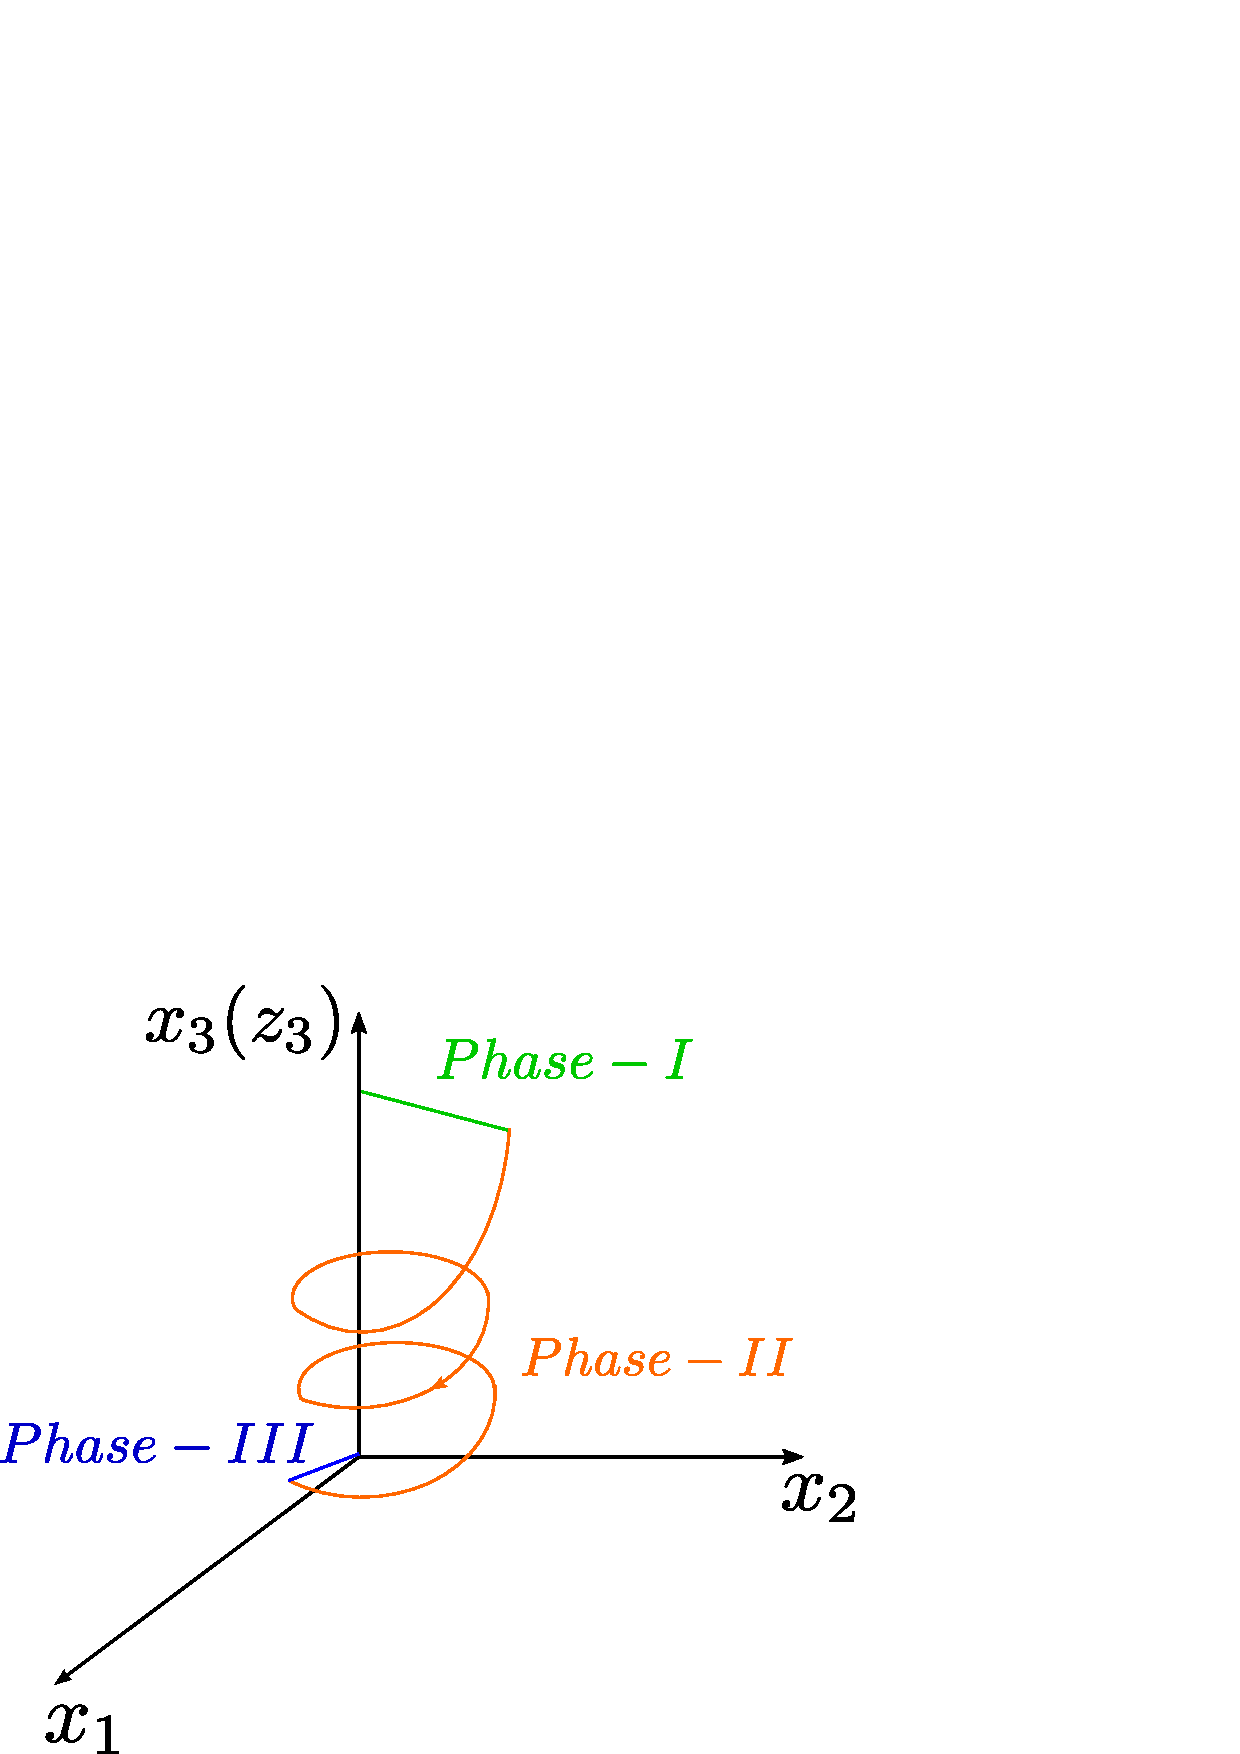
\includegraphics[width=0.4\linewidth]{bild/modul/Schraubenlinie.pdf}%12cm
	\caption{Skizze der Trajektorie des Zustandsvektors mit der Schraubenlinie.}
	\label{fig:Schraubenlinie}
\end{figure}

Wenn $r>0$ läuft die Trajektorie von $\vect{x}$ in Phase-II von $x_{3,0}$ bis zur $X_{1}$-$X_{2}$-Ebene bei $x_{3,0}>0$ abwärts, sonst von unten nach oben. Wenn der Punkt auf der $X_{1}$-$X_{2}$-Ebene weit von der Ruhelage liegt, kann sich der Regler in Phase-III so einstellen lassen, dass $x_{1}$ und $x_{2}$ (oder $r$ in der Zylinderkoordinate) nach und nach bis zu $0$ verkleinern und gleichzeitig $x_{3}$ (oder $z$ in Zylinderkoordinate) noch $0$ bleibt. 

Ein Ausnahme steht in der Situation, wenn der Anfangswert von $\vect{x}$ auf der $z$-Achse liegt. Bei $x_{1,0}$ und $x_{2,0}$ beide $0$ ist der Radius $r_{0}$ auch $0$. Unter der Berücksichtigung der Unveränderlichkeit von $r$ in der ganzen Phase-II ändert sich $\dot{z}$ in Gl. \eqref{eq:Ableitung_r_phi_z_in_Zylinderachse} auch nicht. Deswegen kann die Trajektorie nie nur mittels der vorherigen Idee zur Ruhelage erreichen. Dieses Problem kann man mit dem Entwurf einer zusätzlichen Phase vor Phase-II gelöst werden. Während der Phase-I verändert nur $r$, der am Ende dieser Phase weit von der $z$-Achse liegt.

Und schließlich ergibt sich noch eine Frage: Wie weit muss sich $r$ in Phase-I von $z$-Achse entfernen? Das Problem kann man mit dem kürzesten Weg der gesamten Trajektorie beantworten. Die Länge des Pfads der drei Pahsen ist\footnote{Der detaillierte Rechenverlauf ist in Anhang \ref{Rechenverlauf_fuer_L_Tra} dargestellt}: 
\begin{eqnarray}
L_{Tra} &=& r_1 + \int_{0}^{T_{2}} \sqrt{\dot x_1^2 + \dot x_2^2 + \dot x_3^2 }\, dt + r_1 \notag\\&=& \frac{z_{0}}{r_{1}}\sqrt{r_{1}^{2}+1} + 2r_{1}
\label{eq:Länge_der_Schraubenkurve}
\end{eqnarray} 
wobei die Bogenlänge in Phase-I gleich ist wie in Phase-III und mit $r_{1}$ gekennzeichnet wird. $T_{2}$ steht für die Überführungszeit in Phase-II. Setzt man die Ableitung von $L_{Tra}$ nach $r_{1}$:
\begin{eqnarray}
\frac{\partial L_{Tra}}{\partial r_{1}} = \frac{z_{0}}{\sqrt{r_{1}^{2} + 1}} - \frac{z_{0}}{r_{1}^{2}} \sqrt{r_{1}^{2} + 1} + 2
\label{eq:Ableitung_von_L_Tra}
\end{eqnarray} 
gleich null ein, wird eine von $z_{0}$ abhängigen optimale Bogenlänge in Phase-I $r_{1,opt}$ ausgerechnet, mit der $L_{Tra}$ am kleinsten ist. Wenn der Anfangswert von $r_{0}$ kleiner als $r_{1,opt}$ ist, soll $r$ noch weiter von $z$ entfernen. Im anderen Fall geht das System mit dem Regelgesetz direkt in die Phase-II.

Der nächste Schritt ist der Entwurf von $\vect{u}$ gemäß der obere Idee. Fängt man mit dem Systemeingang in Phase-I an. Wie gerade diskutiert soll nur $r$ innerhalb von diesen Phase verändern werden, dann lässt sich $u_{z}=1$ und $v_{z}=0$ einsetzen. In Phase-II ist es gerade umgekehrt, $u_{z}=0$ und $v_{z}=sign(z)$, sodass der Absolutwert von $z$ immer kleiner wird. Am Ende wenn die Trajektorie schon auf $X_{1}$-$X_{2}$-Ebene sehr nähe liegt, wird der Radius $r$ mit $u_{z}=-1$ und $v_{z}=0$ verkleinert. 

\begin{figure}[!h]
	\centering
	\includegraphics[width=\linewidth]{bild/30_32/Brockett_e2_ck_x.pdf}%13cm
	\caption{Zustandsverläufe mit dem Startwert $(0,5,5)$.}
	\label{fig:Brockett_e2_ck_ein_Fall}
\end{figure}

Dieses Regelgesetz wird auch wieder in zwei Fällen getestet. Der erste ist ähnlich wie dem letzten Abschnitt in Bezug auf \emph{einen} Startwert von $\vect{x}$. Abb. \ref{fig:Brockett_e2_ck_ein_Fall} und \ref{fig:3d_Brockett_e2_ck} zeigen die simulierten Ergebnissen mit $\vect{x}_{0}=(0,0,5)$ und $T_{end}=6s$. Die Ergebnisse entsprechen der Erwartung. $r_{1,opt}$ ist ungefähr $1.29$. Mit $u_{z}/v_{z}=1$ dauern die Phase-I und Phase-III jeweils $1.29s$.
\begin{figure}[!h]
	\centering
	\includegraphics[width=0.8\linewidth]{bild/30_32/3d_Brockett_e2_ck.pdf}%13cm
	\caption{3D-Kurve des Systemzustands mit dem Startwert $(0,5,5)$.}
	\label{fig:3d_Brockett_e2_ck}
\end{figure}

Das zweite Beispiel zielt auf die Prüfung der asymptotischen Stabilität der Ruhelage $(0,0,0)$. Anfangswerte sind eine zufällige Liste mit $20$ Elementen, die in dem Wertebereich $[-0.5,0.5)$ liegen. Der Endzeit $T_{end}=4s$. Als Ergebnis kann die Trajektorie in jedem Fall die Ruhelage erreichen. Die asymptotische Stabilität wird dadurch verifiziert.

\begin{figure}[!h]
	\centering
	\includegraphics[width=\linewidth]{bild/30_32/Brockett_e2_ck_x_Asy.pdf}%13cm
	\caption{Zustandsverläufe mit unterschiedlichen Anfangswerten.}
	\label{fig:Brockett_e2_ck_x_Asy}
\end{figure}

Im Vergleich mit dem Regelgesetz aus Literatur \cite{liberzon2012switching} b.z.w. Abschnitt \ref{Reglerentwurf_für_den_Brocketts_nichtholonomischen_Doppelintegrator_in_Literatur_liberzon2012switching} hat dieses einige Vorteile. Ein wichtiger Punkt liegt in die kürze Konvergenz-Zeit der Trajektorie. Mit gleichen Anfangswerten von $\vect{x}_{0}$ ist die Trajektorie mit dem Regelgesetz in \cite{liberzon2012switching} in $10s$ noch nicht fertig, während die mit diesem Regelgesetz nach $3s$ schon zur Ruhelage ankommt. Die Konvergenzgeschwindigkeit ist deutlich schneller.

Bemerkenswert ist, dass das in drei Phasen schaltende Regelgesetz nicht kontinuierlich ist, nämlich die Brockett Bedingung nicht verletzt. 

Fazit: In diesem Kapitel wurden einige Steuerung und Regler für die Untersuchung der asymptotischen Stabilität der Ruhelage in Brocketts berühmten nicht-holonomen Doppelintegrator vorgestellt. Jeder kann die Trajektorie schließlich in die Ruhelage führen, auch wenn jeder nicht stetig differenzierbar ist. Das steht im Einklang mit Brocketts Bedingungen.